 %----------------------------------------------------------------------------------------
%   Доорх хэсгийг өөрчлөх шаардлагагүй
%----------------------------------------------------------------------------------------
%!TEX TS-program = xelatex
%!TEX encoding = UTF-8 Unicode
\documentclass[12pt,A4]{report}

\usepackage{fontspec,xltxtra,xunicode}
\setmainfont[Ligatures=TeX]{Times New Roman}
\setsansfont{Arial}

% \usepackage[utf8x]{inputenc}
% \usepackage[mongolian]{babel}
%\usepackage{natbib}
\usepackage{geometry}
%\usepackage{fancyheadings} fancyheadings is obsolete: replaced by fancyhdr. JL
\usepackage{fancyhdr}
\usepackage{float}
\usepackage{afterpage}
\usepackage{graphicx}
\usepackage{amsmath,amssymb,amsbsy}
\usepackage{dcolumn,array}
\usepackage{tocloft}
\usepackage{dics}
\usepackage{nomencl}
\usepackage{upgreek}
\newcommand{\argmin}{\arg\!\min}
\usepackage{mathtools}
\usepackage[hidelinks]{hyperref}

\usepackage{algorithm}
\usepackage{algpseudocode}

\usepackage{listings}
\DeclarePairedDelimiter\abs{\lvert}{\rvert}%
\makeatletter
\usepackage{caption}
\captionsetup[table]{belowskip=0.5pt}
\usepackage{subfiles}

\usepackage{listings}
\renewcommand{\lstlistingname}{Код}
\renewcommand{\lstlistlistingname}{\lstlistingname ын жагсаалт}

\usepackage{color}
\definecolor{codegreen}{rgb}{0,0.6,0}
\definecolor{codegray}{rgb}{0.5,0.5,0.5}
\definecolor{codepurple}{rgb}{0.58,0,0.82}
\definecolor{backcolour}{rgb}{0.99,0.99,0.99}
 
\lstdefinestyle{mystyle}{
    basicstyle=\ttfamily\small,
    backgroundcolor=\color{backcolour},   
    commentstyle=\color{codegreen},
    keywordstyle=\color{magenta},
    numberstyle=\tiny\color{codegray},
    stringstyle=\color{codepurple},
    %basicstyle=\footnotesize,
    breakatwhitespace=false,         
    breaklines=true,                 
    captionpos=b,                    
    keepspaces=false,                 
    numbers=left,                    
    numbersep=10pt,                  
    showspaces=false,                
    showstringspaces=true,
    showtabs=false,                  
    tabsize=2
}
 
\lstset{style=mystyle, label=DescriptiveLabel} 

\let\oldabs\abs
\def\abs{\@ifstar{\oldabs}{\oldabs*}}
\makenomenclature
\begin{document}


%----------------------------------------------------------------------------------------
%   Өөрийн мэдээллээ оруулах хэсэг
%----------------------------------------------------------------------------------------

% Дипломийн ажлын сэдэв
\title{DDPG бататгасан сургалтын үйлдлийн шуугианыг турших, харьцуулах }
% Дипломын ажлын англи нэр
\titleEng{Effect of action space noise for DDPG RL algorithm}
% Өөрийн овог нэрийг бүтнээр нь бичнэ
\author{Батбаярын Бямбаням}
% Өөрийн овгийн эхний үсэг нэрээ бичнэ
\authorShort{Б.Бямбаням}
% Удирдагчийн зэрэг цол овгийн эхний үсэг нэр
\supervisor{Г.Гантулга}
% Хамтарсан удирдагчийн зэрэг цол овгийн эхний үсэг нэр
\cosupervisor{}

% СиСи дугаар 
\sisiId{17B1NUM1479}
% Их сургуулийн нэр
\university{МОНГОЛ УЛСЫН ИХ СУРГУУЛЬ}
% Бүрэлдэхүүн сургуулийн нэр
\faculty{ХЭРЭГЛЭЭНИЙ ШИНЖЛЭХ УХААН, ИНЖЕНЕРЧЛЭЛИЙН СУРГУУЛЬ}
% Тэнхимийн нэр
\department{МЭДЭЭЛЭЛ, КОМПЬЮТЕРИЙН УХААНЫ ТЭНХИМ}
% Зэргийн нэр
\degreeName{Бакалаврын судалгааны ажил}
% Суралцаж буй хөтөлбөрийн нэр
\programeName{Мэдээллийн технологи (D061304)}
% Хэвлэгдсэн газар
\cityName{Улаанбаатар}
% Хэвлэгдсэн огноо
\gradyear{2021 оны 02 сар}


%----------------------------------------------------------------------------------------
%   Доорх хэсгийг өөрчлөх шаардлагагүй
%----------------------------------------------------------------------------------------
%----------------------Нүүр хуудастай хамаатай зүйлс----------------------------
\pagenumbering{roman}
\makefrontpage
\maketitle

\doublespace

% Decleration
\begin{huge}
\textbf{Зохиогчийн баталгаа}
\end{huge} \\ \ \\ 
\doublespace
Миний бие \@author \ "\@title" \ сэдэвтэй судалгааны ажлыг гүйцэтгэсэн болохыг зарлаж дараах зүйлсийг баталж байна:
\begin{itemize}
\item Ажил нь бүхэлдээ эсвэл ихэнхдээ Монгол Улсын Их Сургуулийн зэрэг горилохоор дэвшүүлсэн болно.
\item Энэ ажлын аль нэг хэсгийг эсвэл бүхлээр нь ямар нэг их, дээд сургуулийн зэрэг горилохоор оруулж байгаагүй.
\item Бусдын хийсэн ажлаас хуулбарлаагүй, ашигласан бол ишлэл, зүүлт хийсэн.
\item Ажлыг би өөрөө (хамтарч) хийсэн ба миний хийсэн ажил, үзүүлсэн дэмжлэгийг дипломын ажилд тодорхой тусгасан. 
\item Ажилд тусалсан бүх эх сурвалжид талархаж байна. 
\end{itemize} 
\ 

Гарын үсэг: \underline{\hspace{5cm}} 

Огноо: 	\ \ \underline{\hspace{3cm}}

% Гарчгийг автоматаар оруулна
\setcounter{tocdepth}{1}
\tableofcontents

% Зургийн жагсаалтыг автоматаар оруулна
\listoffigures

% Хүснэгтийн жагсаалтыг автоматаар оруулна
\listoftables

% Кодын жагсаалтыг автоматаар оруулна
\lstlistoflistings

% This puts the word "Page" right justified above everything else.
\newpage
%% \addtocontents{lof}{Зураг~\hfill Хуудас \par}
\newpage
%% \addtocontents{lot}{Хүснэгт~\hfill Хуудас \par}

\renewcommand{\cftlabel}{Зураг}

\begin{huge}
\textbf{Товчилсон үг}
\end{huge}
\doublespace

DDPG - Deep Deterministic Policy Gradient

RL - Reinforcement learning

DNN - Deep Neural Network

ANN - Artificial Neural Network

LR - Learning rate

\doublespace
\pagenumbering{arabic}


% Удиртгалыг оруулж ирэх ба abstract.tex файлд удиртгалаа бичнэ
\begin{abstract}
  Reinforcement learning буюу бататгасан сургалтад тасралттай үйлдлийн хувьд суралцах үйл явц нь санамсаргүй үйлдлийг сонгох замаар явагддаг. Харин үргэлжилсэн үйлдлийн хувьд суралцах үйл явц нь үйлдэлд шуугианыг нэмэх замаар явагддаг. Deep Deterministic Policy Gradient (DDPG) бол тасралтгүй, үргэлжилсэн үйлдлүүдийг сурахад зориулагдсан алгоритм тул action space noise буюу үйлдлийн шуугиан ашиглагдана. Энэ судалгааны ажлаар 3 төрлийн шуугианыг харьцуулах, турших бөгөөд ямар үр нөлөөтэй, аль шуугиан нь илүү болохыг тодорхойлно.
  
\section{Зорилго}

DDPG бататгасан сургалтын үйлдлийн шуугианыг туршин, харьцуулж энэ шуугиан моделийг сургах үйл явцад хэрхэн нөлөөлж буйг ажиглан дүгнэлт гаргах

\section{Зорилтууд}

\begin{itemize}
	\item Моделийг DDPG алгоритмыг ашиглан BiPedalWalker-V3 орчныг дуустал алхаж чаддаг болгох
	\item Бие биенээсээ хамааралтай шуугиан, бие биенээсээ хамааралгүй шуугиан, параметр шуугиан гэх гурван төрлийн шуугианыг амжилттай хэрэгжүүлэх
	\item Хэрэгжүүлэлт хийхдээ кодыг аль болох ойлгомжтой DDPG алгоритын pseudo кодын дагуу хэрэгжүүлэх
\end{itemize}
  
\end{abstract}


%----------------------------------------------------------------------------------------
%   Дипломын үндсэн хэсэг эндээс эхэлнэ
%----------------------------------------------------------------------------------------
%\addcontentsline{toc}{part}{БҮЛГҮҮД}
% Шинэ бүлэг

\chapter{Судалгаа}

\section{Бататгасан сургалтын алгоритм}

DDPG алгоритмыг тайлбарлахаас өмнө Reinforcement Learning буюу бататгасан сургалтын талаар бага зэрэг тайлбарлая. Цаашдаа RL гэж товчлон бичнэ.

RL нь агент болон орчин гэсэн хоёр хэсгээс тогтдог. Орчин гэдэг нь агент ажиллаж байгаа объектыг, агент гэдэг нь RL алгоритмыг илэрхийлнэ.

\begin{figure}[H]
\centering
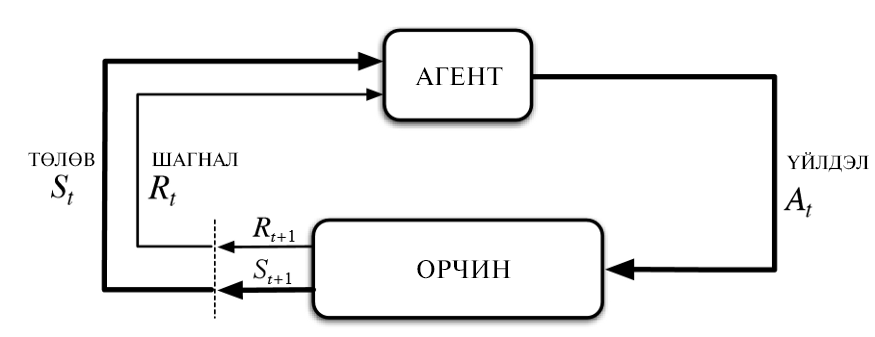
\includegraphics[width=0.8\textwidth]{./images/rl}
\caption{Бататгасан сургалтын бүтэц}
\end{figure}

Орчин нь агентруу төлөвийг илгээх байдлаар эхэлдэг бөгөөд агент нь мэдлэг дээрээ тулгуурлан тухайн нөхцөл байдалд хариу үйлдэл үзүүлнэ. Үүний дараа орчин агент руу дараагийн төлөв болон reward-ыг илгээнэ. Агент нь орчноос хүлээн авсан reward-аар мэдлэгээ шинэчилнэ. Энэ давталт нь орчноос дуусгах төлөв илгээх хүртэл үргэлжилнэ. Ихэнх RL алгоритмууд дээрх байдлаар ажилладаг.

\subsection{Бататгасан сургалттай холбоотай нэр томъёо}

\begin{itemize}
	\item Action (A): Агент-ийн хийх боломжтой бүх алхмууд
	\item State (S): Орчноос буцаж ирэх тухайн нөхцөл байдал
	\item Reward (R): өмнөх үйлдлийн үр дүнд гарсан ололт
	\item Policy (\(\pi\)): Агент одоогийн төлөв байдалд үндэслэн дараагийн үйлдлийг тодорхойлоход ашигладаг стратеги. 
	\item Value (V): урт хугацааны ололт
	\item Q-value эсвэл action-value(Q): Value-тай төстэй. Гэхдээ одоогийн үйлдлийг нэмэлт параметрээр авдаг.
\end{itemize}

\subsection{Model-free}

Model-free гэдэг нь мэдлэгээ шинэчлэхийн тулд шагналд тулгуурладаг. Төлөвүүд болон үйлдлүүдийг хадгалах шаардлагагүй. 

\subsection{On-policy болон off-policy}

On-policy агент нь value-г одоогийн policy-г ашигласан одоогийн үйлдэлд тулгуурлан сурдаг. Харин off-policy агент өөр нэг policy-г ашигласан үйлдэл a*-д тулгуурлан сурдаг.

\subsection{Суралцах үйл явц}

Reinforcement learning буюу бататгасан сургалтад тасралттай үйлдлийн хувьд суралцах үйл явц нь санамсаргүй үйлдлийг сонгох замаар явагддаг. Харин үргэлжилсэн үйлдлийн хувьд суралцах үйл явц нь үйлдэлд шуугианыг нэмэх замаар явагддаг.

\section{Гүн неороны сүлжээ}

Хиймэл неороны сүлжээ (ANN) нь тархи хэрхэн ажилладагаас санаа авсан функцийг ойролцоологч (function approximator) юм. ANN нь нэг давхарга дахь нейронууд бүгд урд давхарга дахь нейронуудтай холбогддог хэд хэдэн давхарласан хиймэл неороноос бүрдэнэ. Бүх хиймэл неоронууд нь идэвхжүүлэх функцтэй байдаг бөгөөд энэ нь ихэвчлэн ReLu функц байдаг. 

\begin{center}
$f(x)=max(0, x)$
\end{center}

$X_j$ нь неоронтой холбогдсон тохиолдолд $w_{ij}$ жинтэй байдаг ба нейрон бүр хэвийх утгатай $b_i$ байдаг. Неороны гаралтыг дараах томъёогоор тооцоолж болно:

\begin{center}
$y=f(b_i+\sum_{h=1}^{n}w_{ij} x_j)$
\end{center}

Эхний давхаргыг оролт болгон ашигласнаар оролтыг өөр давхаргаар дамжуулж, сүлжээний сүүлийн давхаргаас гарах утгыг авах боломжтой. ANN нь илүү нарийн төвөгтэй функцуудыг ойролцоолох боломжтой тохиромжтой олон давхарга, неоронуудтай бол гүн неороны сүлжээ (DNN) гэж үздэг. 

\section{DDPG алгоритм}

Deep Deterministic Policy Gradient (DDPG) бол үргэлжилсэн, тасралтгүй үйлдлүүдийг сурахад зориулагдсан model-free off-policy алгоритм юм. Q-функц ба policy-ыг зэрэг сурдаг алгоритм юм. Q-функцийг сурахын тулд off-policy өгөгдөл болон Bellman тэгшитгэлийг ашигладаг. Мөн policy-г сурахын тулд Q-функцыг ашигладаг. 

DDPG алгоритм дараах 4 неороны сүлжээг ашигладаг:
\begin{itemize}
	\item ${\theta}^Q$:Actor сүлжээ
	\item ${\theta}^{\mu}$:Critic сүлжээ
	\item ${\theta}^{Q^{'}}$:target Actor сүлжээ
	\item ${\theta}^{{\mu}^{'}}$:target Critic сүлжээ
\end{itemize} 
 
Actor сүлжээ нь төлөвөөс хамааран үйлдлийг санал болгоно. Төлөвийг оролтоор авч үйлдлийг гаргана. Critic сүлжээ нь төлөвөөс хамаарсан үйлдэл нь сайн эсвэл муу болохын урьдчилан таамагладаг. Төлөв болон үйлдлийг оролтоор авч Q-value-г гаргадаг.

Target network нь суралцсан сүлжээнүүдийг хянаж байдаг эх сүлжээнүүдийнхээ хуулбарууд юм. Эдгээр сүлжээг ашиглан тогтвортой сурах байдлыг сайжруулдаг.	

Доор DPDG алгоритмын pseudo-code-ыг харууллаа. Үүнийг 4 хэсэгт задлан тайлбарлаж болно.

\begin{itemize}
	\item Туршлагаа хадгалах (Experience replay)
	\item Actor болон critic сүлжээг шинэчлэх
	\item Target сүлжээг шинэчлэх
	\item Судалгаа хийх (Exploration)
\end{itemize} 

------------------------------------------------------------------------------------------------------------------
DDPG алгоритмын pseudo code

------------------------------------------------------------------------------------------------------------------
$\theta^Q$ болон $\theta^{\mu}$ жинтэйгээр critic сүлжээ $Q(s_i,a_i|\theta^Q)$ болон actor сүлжээ $\mu(s|\theta^mu)$ -г үүсгэнэ

$\theta^{Q{'}} \longleftarrow \theta^Q$, $\theta^{\mu{'}} \longleftarrow \theta^\mu$ жинтэйгээр target сүлжээ $Q^{'}$ болон $\mu^{'}$-г үүсгэнэ

Replay buffer-aa үүсгэнэ

for episode = 1, M do

\quad Анхны төлөв болох s1-г авна

\quad for t = 1, T do

\quad\quad Тухайн policy болон шуугиан дээрээ үндэслэн үйлдлээ сонгоно $a_t = \mu(s_t|\theta^\mu)+N_t$

\quad\quad Үйлдэл $a_t$-гээ гүйцэтгээд reward $r_t$ болон шинэ төлөв $s_t+1$-ээ авна

\quad\quad Replay buffer-даа төлөв, үйлдэл, reward, шинэ төлөвөө ($s_t, a_t, r_t, s_t+1$) хадгалж авна

\quad\quad Replay buffer-аасаа N тооны санамсаргүй утгыг авна

\quad\quad $y_i=r_i+\gamma{Q^{'}}(s_i+1,\mu^{'}(s_i+1|\theta^{\mu^{'}})|\theta^{Q{'}})$ утгыг онооно

\quad\quad Loss-ыш багасгаж critic сүлжээг шинэчилнэ: $L = \dfrac{1}{N}\sum_{i}(y_i-Q(s_i,a_i|\theta^Q))^2$

\quad\quad Actor policy-г шинэчлэнэ: 
\begin{center}
$\bigtriangledown_\theta\mu J(\theta) \approx \dfrac{1}{N}\sum_{i}[\bigtriangledown_a Q(s, a|\theta^Q)|_s=s_i,a=\mu(s_i)\bigtriangledown_\theta\mu \mu(s|\theta^\mu)|_s=s_i]$
\end{center}

\quad\quad Target сүлжээнүүдийг шинэчлэнэ:
\begin{center}
$\theta^{Q{'}} \longleftarrow \tau\theta^Q + (1-\tau)\theta^{Q{'}}$ 

$\theta^{\mu{'}} \longleftarrow \tau\theta^\mu + (1-\tau)\theta^{\mu{'}}$ 
\end{center}

\quad\quad end for

\quad end for

\subsubsection{Replay buffer}

DDPG алгоритм нь replay buffer-ыг туршлагыг цуглуулахад ашигладаг. Цуглуулсан туршлагаа неороны сүлжээний параметрүүдийг шинэчлэхэд ашигладаг. Value болон policy сүлжээг шинэчлэхдээ replay buffer дахь туршлагуудаас санамсаргүй байдлаар цуглуулан ашигладаг.

Яагаад replay buffer-ыг ашиглаж байгаа вэ гэхээр алгоритмд хамааралгүй байдлаар тархсан өгөгдөл хэрэгтэй. Ийм өгөгдлүүдийг replay buffer дахь туршлагуудаас санамсаргүй байдлаар сонгон авах байдлаар цуглуулж болно.

\subsubsection{Actor болон Critic сүлжээг шинэчлэх}

Critic сүлжээг шинэчлэх үйл явц нь Q-learning-тэй төстэй байдлаар хийгддэг. Шинэчлэгдсэн Q утгыг Беллманы тэгшитгэлээс гарган авна:

\begin{center}
$y_i=r_i+\gamma{Q^{'}}(s_i+1,\mu^{'}(s_i+1|\theta^{\mu^{'}})|\theta^{Q{'}})$
\end{center}

DDPG-д дараагийн төлөв Q утгуудыг target critic network, target actor network ашиглан тооцдог. Дараа нь шинэчлэгдсэн Q утга ба анхны Q утга хоорондын дундаж квадрат алдааг хамгийн бага хэмжээнд хүртэл бууруулна:

\begin{center}
$Loss = \dfrac{1}{N}\sum_{i}(y_i-Q(s_i,a_i|\theta^Q))^2$
\end{center}

Анхны Q утга нь target network-оос биш critic network-оос бодогдон гарна. 

Actor сүлжээний хувьд гол зорилго нь буцан ирэх үр дүн хамгийн дээд хэмжээнд байх юм:

\begin{center}
$J(\theta) = E[Q(s, a)|_s=s_t,a_t=\mu(s_t)]$
\end{center}

Actor алдагдлыг тооцоолохын тулд зорилгын функцийн деривативыг авна:

\begin{center}
$\bigtriangledown_\theta\mu J(\theta) \approx \bigtriangledown_a Q(s, a)\bigtriangledown_\theta\mu \mu(s|\theta^\mu)$
\end{center}

Policy-гоо off-policy байдлаар шинэчилж байгаа учир санамсаргүй байдлаар авсан туршлагуудынхаа градиентүүдийн нийлбэрийн дундаж утгыг авна:

\begin{center}
$\bigtriangledown_\theta\mu J(\theta) \approx \dfrac{1}{N}\sum_{i}[\bigtriangledown_a Q(s, a|\theta^Q)|_s=s_i,a=\mu(s_i)\bigtriangledown_\theta\mu \mu(s|\theta^\mu)|_s=s_i]$
\end{center}

\subsubsection{Target сүлжээг шинэчлэх}
 
Target сүлжээний параметрүүдийг хуулбарлаад, тэдгээрээр дамжуулан сурсан сүлжээнүүдээ хянана. Target сүлжээний параметрүүдийг тодорхой хугацааны алхам хийсний дараа дараах томъёогоор шинэчилдэг:

\begin{center}
$\theta^{Q{'}} \longleftarrow \tau\theta^Q + (1-\tau)\theta^{Q{'}}$ 

$\theta^{\mu{'}} \longleftarrow \tau\theta^\mu + (1-\tau)\theta^{\mu{'}}$ 

$\tau $ бол ихэвчлэн 1-тэй ойролцоо байхаар сонгосон параметр юм (жишээлбэл: 0.999).
\end{center}

\subsubsection{Шуугиан нэмэх}

DDPG алгоритмын баримт бичиг зохиогчид үйлдэлд шуугиан нэмэхийн тулд N:Ornstein-Uhlenbeck Process-г ашигласан байна:

\begin{center}
$\mu^{'}(s_t) = \mu(s_t|\theta_t^\mu) + N$
\end{center}

Ornstein-Uhlenbeck процесс нь өмнөх шуугиантай уялдаатай холбоотой шуугианыг бий болгодог.

\section{Хиперпараметрүүдийн тохируулга}

RL алгоритмууд нь алгоритм хэрхэн ажиллахыг өөрчилдөг параметрүүд болох хиперпараметрүүдтэй байдаг. Алгоритм нь тодорхой орчинд сайн ажиллаж байгаа эсэхийг баталгаажуулахын тулд хиперпараметрын өөр өөр утгыг ашиглан туршиж аль хиперпараметрүүд нь хамгийн сайн ажиллаж байгаа болохыг олж мэдэхийн тулд хиперпараметрын тохируулга хийх шаардлагатай байдаг.  

\section{Орчны шуугиан}


 
\section{Ашигласан технологи}

\subsection{Gym}

Gym бол reinforcement learning буюу бататгасан сургалтын алгоритмуудыг хөгжүүлэх болон харьцуулахад зориулагдсан хэрэгсэл юм. Үүнийг ашиглан агентдаа алхах, тоглоом тоглох зэрэг бүх зүйлийг зааж болно. 

\subsubsection{Яагаад үүнийг ашигладаг вэ?}

Бататгасан сургалт (RL) нь шийдвэр гаргахтай холбоотой машин сургалтын дэд талбар юм. Энэ нь агент нарийн төвөгтэй, тодорхойгүй орчинд хэрхэн зорилгодоо хүрч болохыг судалдаг. RL нь доорх 2 шалтгааны улмаас ихээр ашиглагдаж байна:

\begin{itemize}
	\item RL нь дараалсан шийдвэр гаргахтай холбоотой бүхий л асуудлыг багтаасан байдаг. Жишээ нь роботын хөдөлгүүрийг удирдаж түүнийг үсрэх чадвартай болгох, үнэ, бараа материалын менежмент гэх мэт бизнесийн шийдвэр гаргах, видео тоглоом, ширээний тоглоом тоглох гэх мэт
	\item RL алгоритмууд олон хүнд хэцүү орчинд сайн үр дүнд хүрч эхэлсэн
\end{itemize} 

Гэсэн хэдий ч RL судалгааны ажлыг RL-ын open-source орчин хангалттай олон янз байдаггүй бөгөөд тэдгээрийг тохируулах, ашиглахад хэцүү байдал болон орчны стандартчилал дутмаг гэсэн хоёр хүчин зүйл удаашруулж байна. Gym нь эдгээр 2 асуудлыг шийдэхийг зоридог.

\subsection{BiPedalWalker-v2}

Энэ бол gym-ын Box2D симулятор дахь нэг орчин юм. Гол зорилго нь bipedal роботыг алхаж сургах. Урагш алхах бүрд reward өгдөг. Нийтдээ төгсгөл хүртэл 300+ оноог өгдөг. Хэрэв робот унавал -100 оноо өгдөг. Илүү сайн агент нь илүү сайн оноо авах болно. 

Төлөв нь их биений өнцгийн хурд, өнцгийн хурд, хэвтээ хурд, босоо хурд, хөлний байрлал, хөлний өнцгийн хурд, хөлтэй газар шүргэлцэх, 10 лидарын зай хэмжигч хэмжигдэхүүнээс бүрдэнэ. Мужийн векторт координат байхгүй байна.

\subsection{Pytorch}

Pytorch бол Torch сан дээр тулгуурласан open-source машин сургалтын сан юм. Python хэлэнд ихээр ашиглагддаг ч мөн С++ програмчлалын хэлд ашиглагддаг. Энэ нь GPU ашигладаг. PyTorch нь өндөр түвшний хоёр онцлог шинж чанарыг агуулдаг:

\begin{itemize}
	\item GPU-г ашиглан тензорын тооцоолол хийх (NumPy гэх мэт) 
	\item Гүнзгий неороны сүлжээг (Deep neural network) бий болгох
\end{itemize}

2016 оны 1 сард гарсан бөгөөд үүнээс хойш олон судлаачид үүнийг ашигласаар байна. Учир нь маш нарийн төвөгтэй неороны сүлжээг хялбараар бий болгодог. Мөн кодоо шалгахдаа заавал бүхлээр нь ажиллуулах шаардлагагүй болсон. Шаардлагатай тохиолдолд Pytorch-ын функцуудыг NumPy, SciPy, Cython зэргээр өргөтгөж болно. 
 
\chapter{Хэрэгжүүлэлт}

\section{Алгоритмын хэрэгжүүлэлт}

Хэрэгжүүлэлтийг python програмчлалын хэлийг ашиглан гүйцэтгэсэн. Орчинг бэлдэхдээ gym openai хэрэгслийг ашигласан. Pytorch санг тооцоолол хийх, неороны сүлжээ үүсгэх зэрэгт ашигласан. Дээр дурдсан DDPG алгоритмын pseudo кодын дагуу кодыг бичсэн. Кодыг хавсралт хэсэг оруулсан. Github-аас үзэхийг хүсвэл дараах холбоосоор хандана уу \url{https://github.com/bbyambanyam/ddpg_algorithm.git}

\section{Алгоритмын турших орчин}

BipedalWalker-v3 орчин дээр алгоритмыг ажиллуулан туршилаа.

\begin{figure}[H]
\centering
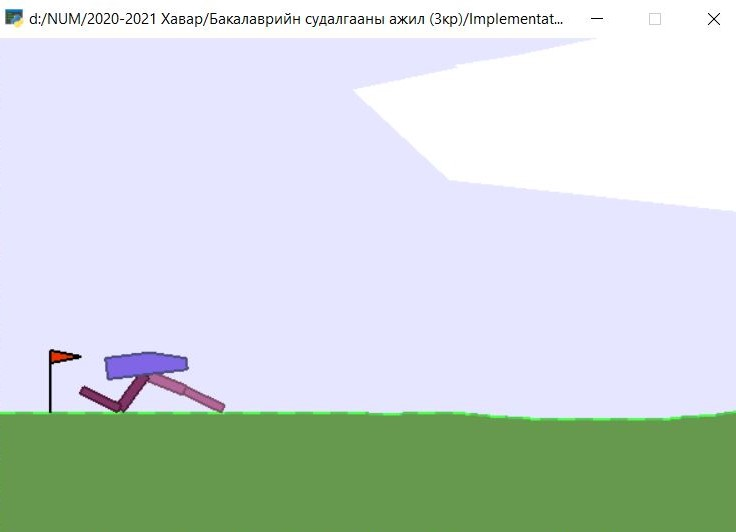
\includegraphics[width=0.8\textwidth]{./images/bipedalwalker}
\caption{BiPedalWalker-V3 орчин}
\end{figure}

Орчинг үүсгэж төлөвийн хэмжээс, үйлдлийн хэмжээс, хийж болох үйлдлийн тоог авна.

\begin{lstlisting}[language=Python, caption=Орчин үүсгэх, frame=single]
env = gym.make('BipedalWalker-v3')

state_dimension = env.observation_space.shape[0]
action_dimension = env.action_space.shape[0]
action_max = env.action_space.high[0]
\end{lstlisting}

\subsection{Хипер параметрүүд}

Доорх DDPG-ийн хипер параметрүүд нь BiPedalWalker-V3 орчныг шийдвэрлэхэд тохируулагдсан болно.

\begin{itemize}
	\item Actor learning rate: 0.0001 (Adam optimizer)
	\item Critic learning rate: 0.0001 (Adam optimizer)
	\item Memory buffer size: 1000000
	\item Minibatch size: 128
	\item OU-noise-theta: 0.15
	\item OU-noise-sigma: 0.2
	\item OU-noise-mu: 0
	\item normal-noise: 0.2
	\item Steps: 1600
	\item Target update: 0.001
\end{itemize}

\section{Чухал кодын хэсгүүд}

Actor, target actor, critic болон target critic сүлжээг optimizer (сургагч)-ын хамт үүсгэх. Үүсгэхдээ төлөвийн хэмжээс, үйлдлийн хэмжээс, хийж болох үйлдлийн тоо зэргийг ашиглана.

\begin{lstlisting}[language=Python, caption=Actor critic сүлжээ үүсгэх, frame=single]
actor = models.Actor(state_dimension, action_dimension, action_max)
target_actor = models.Actor(state_dimension, action_dimension, action_max)
actor_optimizer = torch.optim.Adam(actor.parameters(), lr=0.001)

critic = models.Critic(state_dimension, action_dimension)
target_critic = models.Critic(state_dimension, action_dimension)
critic_optimizer = torch.optim.Adam(critic.parameters(), lr=0.001)

for target_param, param in zip(target_actor.parameters(), actor.parameters()):
	target_param.data.copy_(param.data)

for target_param, param in zip(target_critic.parameters(), critic.parameters()):
    target_param.data.copy_(param.data)
\end{lstlisting}

Replay buffer үүсгэх.

\begin{lstlisting}[language=Python, caption=Replay buffer үүсгэх, frame=single]
ram = memory.ReplayBuffer(1000000))
\end{lstlisting}

Action noise-г үүсгэхдээ Ornstein-Uhlenbeck Process-г ашигласан

\begin{lstlisting}[language=Python, caption=Шуугиан үүсгэх, frame=single]
noise = utilities.OrnsteinUhlenbeckActionNoise(action_dimension)
\end{lstlisting}

Үйлдэл дээр correleted шуугианыг нэмэх

\begin{lstlisting}[language=Python, caption=Үйлдэл дээр шуугиан нэмэх, frame=single]
action_with_noise = action_without_noise.data.numpy() + (noise.sample() * action_max)
\end{lstlisting}

Үйлдэл дээр uncorreleted шуугианыг нэмэх

\begin{lstlisting}[language=Python, caption=Үйлдэл дээр шуугиан нэмэх, frame=single]
action_with_noise = action_without_noise.data.numpy() + (random.uniform(-0.2, 0.2) * action_max)
\end{lstlisting}

Үйлдлийг хийж шинэ төлөв, reward-г авах

\begin{lstlisting}[language=Python, caption=Үйлдэл хийх, frame=single]
new_observation, reward, done, info = env.step(action_with_noise)
\end{lstlisting}

Critic сүлжээг сургаад, шинэчлэх

\begin{lstlisting}[language=Python, caption=Critic сүлжээг сургах шинэчлэх, frame=single]
# Critic network-g surgah

predicted_action = target_actor.forward(next_states).detach()
next_val = torch.squeeze(target_critic.forward(next_states, predicted_action).detach())
y_expected = rewards + 0.99*next_val
y_predicted = torch.squeeze(critic.forward(states, actions))

# Critic network-g shinechleh, critic loss-g tootsooloh
            
critic_loss = F.smooth_l1_loss(y_predicted, y_expected)
critic_optimizer.zero_grad()
critic_loss.backward()
critic_optimizer.step()
\end{lstlisting}	

Actor сүлжээг сургах

\begin{lstlisting}[language=Python, caption=Actor сүлжээг сургах, frame=single]
predicted_action = actor.forward(states)
actor_loss = -1*torch.sum(critic.forward(states, predicted_action))
actor_optimizer.zero_grad()
щactor_loss.backward()
щactor_optimizer.step()
\end{lstlisting}

\chapter{Үр дүнгийн боловсруулалт}

\section{Туршилтын үр дүн}

Хэрэв алгоритм зөв ажиллаж байгаа бол reward нь өсөж байх ёстой байдаг. Дундаж reward-ыг авахдаа episode болгоны нийлбэр reward-г олоод үүнийгээ list-д хадгалан аваад энэ list-ээс сүүлийн 40 үр дүнгийн дундажыг олж графикийг зурсан.

\subsection{Үйлдлийн орчны шуугиан}

\subsubsection{Correlated шуугиан}

Доорх графикийн хувьд 800 episode ажилласан бөгөөд босоо тэнхлэгийн дагуу дундаж reward, хэвтээ тэнхлэгийн дагуу ажилласан episode-г авч байна. Орчны шуугианыг нэмэхдээ Ornstein-Uhlenbeck Process-г ашигласан. Энэ процесс нь өмнөх шуугиантай уялдаа хамааралтай буюу correlated шуугианыг гаргаж өгнө.

\begin{figure}[H]
\centering
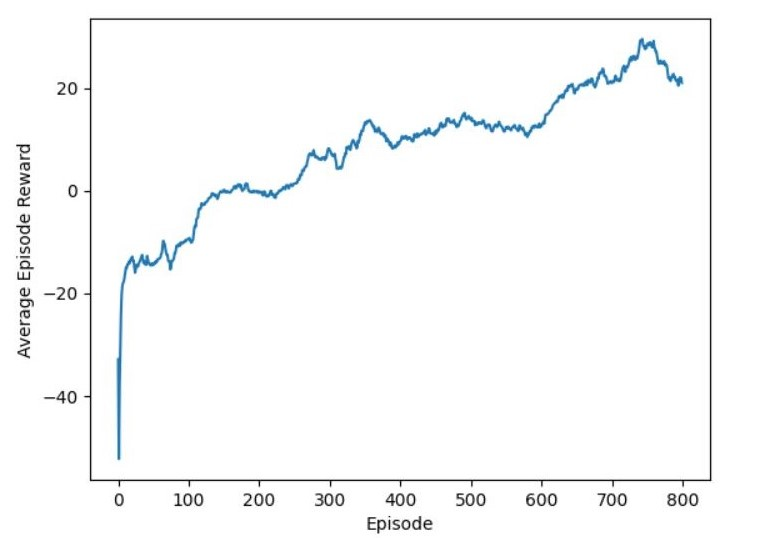
\includegraphics[width=0.7\textwidth]{./images/after_800_ep}
\caption{Correlated noise}
\end{figure}

1000 episode ажиллуулсны дараа:

\begin{figure}[H]
\centering
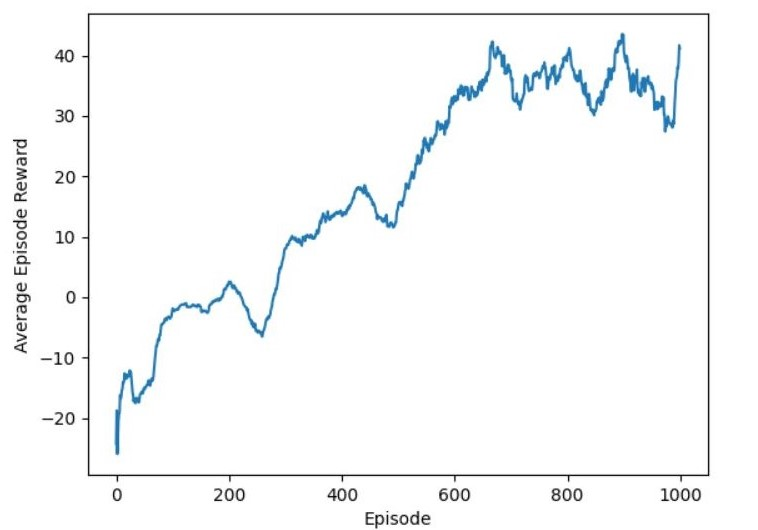
\includegraphics[width=0.7\textwidth]{./images/after_1000_ep2}
\caption{Correlated noise}
\end{figure}

\subsubsection{Uncorrelated шуугиан}

Доорх хоёр графикийн хувьд 800 episode ажилласан бөгөөд орчны шуугианыг -0.2 оос 0.2-ын хооронд санамсаргүй байдлаар сонгон авч үйлдэл дээрээ нэмж байгаа. Энэ нь өмнөх шуугиантай уялдаа хамааралгүй буюу uncorrelated шуугиан гэсэн үг юм. 

\begin{figure}[H]
\centering
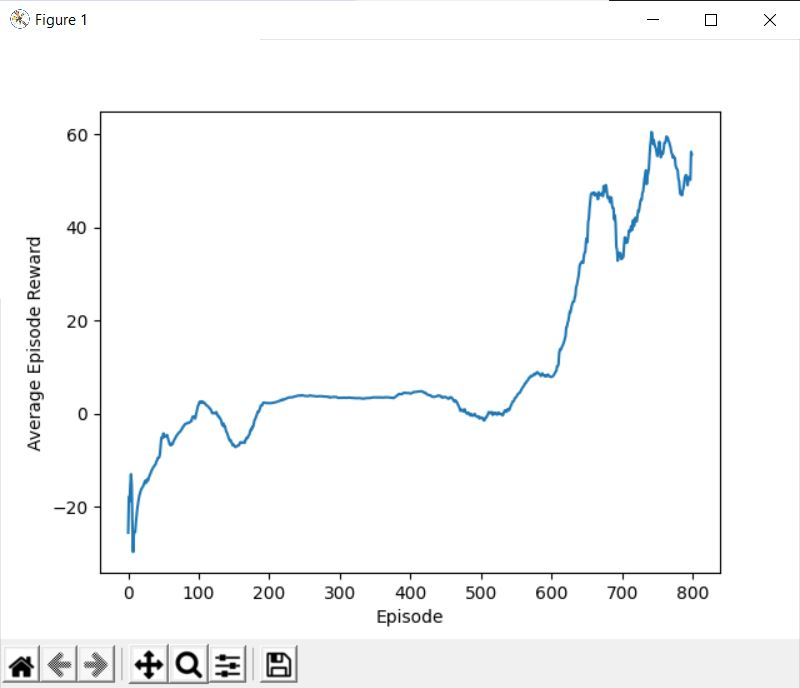
\includegraphics[width=0.8\textwidth]{./images/after_800_ep_02}
\caption{Uncorrelated noise}
\end{figure}

Uncorreleted шуугианы өөр нэг график

\begin{figure}[H]
\centering
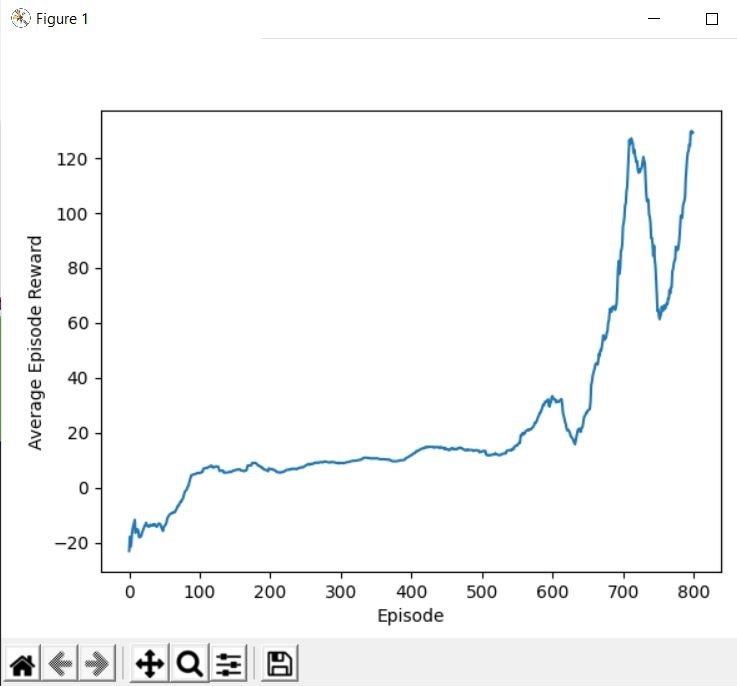
\includegraphics[width=0.8\textwidth]{./images/after_800_ep_02_am}
\caption{Uncorrelated noise 2}
\end{figure}

Доорх графикийн хувьд 800 episode ажилласан бөгөөд орчны шуугианыг -0.4-оос 0.4-ын хооронд санамсаргүй байдлаар сонгон авч үйлдэл дээрээ нэмж байгаа. Энэ нь мөн адил өмнөх шуугиантай уялдаа хамааралгүй буюу uncorrelated шуугиан юм. Графикаас харахад 0.4 өөр сонгон авсан үед нь үр дүн муу гарч байна.

\begin{figure}[H]
\centering
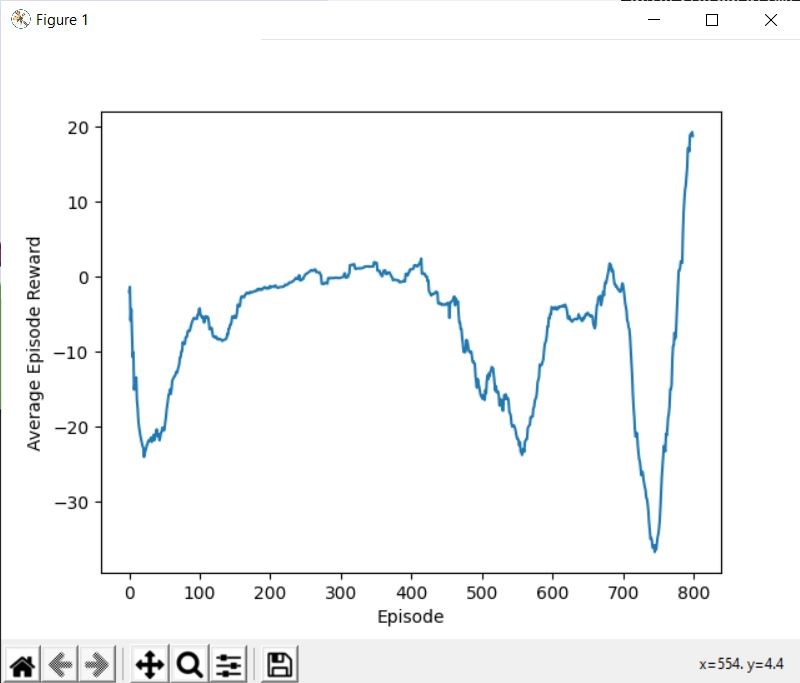
\includegraphics[width=0.8\textwidth]{./images/after_800_ep_04}
\caption{Uncorrelated noise 0.4}
\end{figure}

\subsection{Parameter Space Noise}

\section{Үр дүнгийн харьцуулалт}


%----------------------------------------------------------------------------------------
%   Дүгнэлт эндээс эхэлнэ
%----------------------------------------------------------------------------------------
\conclusion{Дүгнэлт}
Дүгнэлтийг энд бич

%----------------------------------------------------------------------------------------
%   Дипломын номзүй, хавсралтын хэсэг эндээс эхэлнэ
%----------------------------------------------------------------------------------------

\singlespace
\addcontentsline{toc}{part}{НОМ ЗҮЙ}
\begin{thebibliography}{}
	% Ашигласан материалыг эндээс оруулна
	\bibitem{image1}
	Deep Deterministic Policy Gradients Explained, TowardsDataScience, \url{https://towardsdatascience.com/deep-deterministic-policy-gradients-explained-2d94655a9b7b}
	\bibitem{pharagraph1}
	Deep Deterministic Policy Gradient (DDPG),  Keras, \url{https://keras.io/examples/rl/ddpg_pendulum/}
	\bibitem{format1}
	Deep Deterministic Policy Gradient, Spinning Up, \url{https://spinningup.openai.com/en/latest/algorithms/ddpg.html}
	\bibitem{list}
	Continuous Control With Deep Reinforcement Learning, Lillicrap et al 2015, \url{https://arxiv.org/pdf/1509.02971.pdf}
\end{thebibliography}


%----------------------------------------------------------------------------------------
%   Хавсралтууд эндээс эхэлнэ
%----------------------------------------------------------------------------------------
\appendix
\addcontentsline{toc}{part}{ХАВСРАЛТ}

% Хавсралтын нэр. Хавсралт гэдэг үг агуулахгүй
\chapter{А}
Хавсралтын агуулга

% Хавсралтын нэр. Хавсралт гэдэг үг агуулахгүй
\chapter{Кодын хэрэгжүүлэлт}

\end{document}
